\documentclass[11pt]{article}
%\documentclass{siamart0216}

\usepackage{amssymb}
\usepackage{amsmath}
\usepackage{graphicx}
\usepackage{caption}
\usepackage{subcaption}
\usepackage{caption}
\usepackage{float}
\usepackage{subcaption}
\usepackage{dcolumn}
\usepackage{amsthm}
\usepackage{multirow}
\usepackage{enumitem}
\usepackage{amsfonts}
\usepackage{color}

\usepackage[sort]{cite}

% Tikz stuff
\usepackage{pgf}
\usepackage{tikz}
\usetikzlibrary{decorations.pathmorphing}
\usetikzlibrary{arrows.meta,decorations.pathmorphing,backgrounds,positioning,fit}
\usetikzlibrary{shapes,snakes}
\usetikzlibrary{calc}
\tikzset{snake it/.style={decorate, decoration=snake}}

% Number equations by section
\numberwithin{equation}{section}

% Define new commands
\def\Line(#1,#2)(#3,#4){\qbezier(#1,#2)(#1,#2)(#3,#4)}

\newcommand\numberthis{\addtocounter{equation}{1}\tag{\theequation}}
\newcommand{\myfont}{\fontfamily{pcr}\selectfont}
\newcommand{\rpm}{\raisebox{.2ex}{$\scriptstyle\pm$}}
\newcommand{\tribar}{\vert \!  \vert \!  \vert }
\newcommand{\pdrv}[1]{\frac{\partial#1}{\partial t}}
\newcommand{\ddt}[1]{\frac{\partial}{\partial t}#1}
%\newcommand{\inp}[2][]{\left(#1,\, #2\right)}
\newcommand{\inp}[2][]{\left(#1, #2\right)}
%\newcommand{\gnp}[2][]{\langle#1,\, #2\rangle}
\newcommand{\gnp}[2][]{\langle#1, #2\rangle}

\newtheorem{remark}{Remark}[section]
\newtheorem{lemma}{Lemma}[section]
\newtheorem{corollary}{Corollary}[section]
\newtheorem{theorem}{Theorem}[section]
\newtheorem{definition}{Definition}[section]

% Highlight in red
\def\red{\color{red}}

% Calligraphic
\def\Tc{\mathcal{T}}
\def\Ac{\mathcal{A}}
\def\Qc{\mathcal{Q}}
\def\Mc{\mathcal{M}}
\def\Ec{\mathcal{E}}
\def\BDM{\mathcal{BDM}}
\def\BDDF{\mathcal{BDDF}}
\def\RT{\mathcal{RT}}
\def\SS{\mathcal{SS}}
\def\Pc{\mathcal{P}}

% Math bold
\def\X{\mathbb{X}}
\def\W{\mathbb{W}}
\def\R{\mathbb{R}}
\def\M{\mathbb{M}}
\def\S{\mathbb{S}}
\def\N{\mathbb{N}}
\def\I{\mathbb{I}}
\def\H{\mathbb{H}}

% Greeks
\def\s{\sigma}
\def\t{\tau}
\def\g{\gamma}
\def\c{\chi}
\def\l{\lambda}
\def\m{\mu}
\def\z{\zeta}
\def\tet{\theta}
\def\del{\delta}

% Bolds
\def\r{\mathbf{r}}

% Matrices
\def\As{A_{\s\s}}
\def\Au{A_{\s u}}
\def\Ag{A_{\s\g}}

% Hats
\def\Eh{\hat{E}}
\def\Ah{\hat{A}}
\def\Th{\hat{T}}
\def\PIh{\hat{\Pi}}
\def\Qch{\hat{\Qc}}
\def\Qh{\hat{\Qc}}
\def\Mh{\hat{M}}
\def\rh{\hat{\r}}
\def\eh{\hat{e}}
\def\wh{\hat{w}}
\def\qh{\hat{q}}
\def\nh{\hat{n}}
\def\uh{\hat{u}}
\def\vh{\hat{v}}
\def\xh{\hat{x}}
\def\yh{\hat{y}}
\def\sh{\hat{\s}}
\def\th{\hat{\t}}
\def\gh{\hat{\g}}
\def\xih{\hat{\xi}}
\def\ch{\hat{\c}}
\def\teth{\hat{\tet}}
\def\delh{\hat{\del}}
\def\Xh{\hat{\X}}
\def\Vh{\hat{V}}
\def\Wh{\hat{W}}
\def\Ath{\widehat{A\t}}
\def\Acth{\widehat{\Ac\t}}

% Operators
\def\asym{\operatorname{as\,}}
\def\tr{\operatorname{tr\,}}

% Projectors
\def\Quh{Q^{u}_h}
\def\Qgh{Q^{\g}_h}

\def\skew{\operatorname{Skew}}
\def\vec{\operatorname{Vec}}

\def\curl{\operatorname{curl}}
\def\dvr{\operatorname{div}}          % as nabla
\def\dvrg{\operatorname{div}}  % as a word

% Smth
\def\dfi{DF_E^{-1}}
\def\jfi{J_{F^{-1}_E}}

% Boundaries and domains
\def\O{\Omega}
\def\Gn{\Gamma_N}
\def\Gd{\Gamma_D}

% Change margins
\usepackage{geometry}
\geometry{
	letterpaper,
	%	a4paper,
	%	total={210mm,297mm},
	left=20mm,
	right=20mm,
	top=20mm,
	bottom=20mm,
	bindingoffset=0mm
}
\title{The Battle of Neighborhoods: Exploration of Austin Food Venues}
\date{\today}
\begin{document}
\maketitle

%%%%%%%%%%%%%%%%%%%%%%%%%%%%%%%%%%%%%%%%%%%%%%%%%%%%%%%%%%%%%%%%%%
\section{Introduction}
	Located in Texas, Austin is one of the most rapidly growing cities in the United States. According to Census Bureau estimates released in mid-April 2019	 \cite{census}, the Austin-Round Rock metro's population reached 2,168,000 as of July 1, 2018, which resulted in 2.5\% jump from the previous year. The city of Austin also showed a 26.3\% increase in population since 2010 and is now ranked as 11-th largest in the country. According to the newest forecasts, \cite{culture_map}, this trend will only continue and Austin, with the population of 981,035 on January 1, 2019, will reach 1 million by 2020. 
\begin{figure}[ht!]
	\centering
	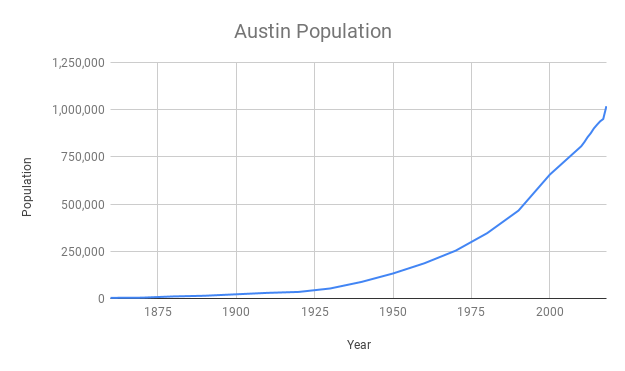
\includegraphics[width=.6\textwidth]{pics/austin_growth}
		\label{fig:1_1}
	\caption{Dynamics of Austin city population}
	\label{fig:4}
\end{figure}
	
	Despite fast-paced growth, the city does not suffer from increasing crime and poverty rates. Indeed,  U.S. News \& World Report, \cite{realestate}, recently ranked Austin as the best place to live in the United States with an overall score of 7.8 out of 10. Steady job growth, stable housing market, and the desirable lifestyle of the city, not to mention {\it the booming tech industry} , have been the reasons to move for many people in places like California, metro Chicago area and New York.
	
Millennials and retiring baby boomers are now making up the majority of new Austinites, all being drawn in for the city's shopping, museums, entertainment, and, last but not the least, restaurants. Austin is of course synonymous with barbecue, as well as killer bars, and all manner of food trucks. And while several years ago the idea of traveling here solely for great restaurants would have been strange, Austin is now becoming one of the top food destination in the US, \cite{zagat}. This, together with city's demographic trends suggests a great opportunity for a new business: {\it open a restaurant, which would feature a more elegant selection of food and drinks, comparing to BBQ, tacos and beer, that at the same time would be interesting and attractive for both locals and tourists.}

{\bf The purpose of this project is to conduct the analysis of Austin food venues and suggest the best unusual category for a new restaurant, together with the optimal location, based on the additional analysis of the city's neighborhoods. }

%%%%%%%%%%%%%%%%%%%%%%%%%%%%%%%%%%%%%%%%%%%%%%%%%%%%%%%%%%%%%%%%%%
\section{Data}
%
\subsection{Data sources}
In order to answer the proposed question, two types of information were required: 
\begin{enumerate}
\item Data, describing the current food venues available in the city. Such information is used in the analysis to discover the most and the least represented, unusual, categories. Furthermore, more detailed information about the unusual restaurants, such as rating, is used to determine the optimal category for a new restaurant. All the required data is obtained through the Foursquare API, \cite{foursquare}.
\item Data, summarizing the geographical representation of the city itself, including the list of its neighborhoods, together with the their coordinates, as well as some extra information, such as each neighborhood's area and population. City-Data website, \cite{city_data}, provides general information and is used to collect data about Austin's neighborhoods.  Further, areaConnect website,  \cite{area_connect}, is used for translating neighborhoods' zipcodes into the corresponding geographical coordinates.
\end{enumerate}
%
\subsection{Neighborhoods data wrangling}
The neighborhoods data was scraped using requests and BeautifulSoup libraries. The starting point was the City-Data website main page, that looks as following:
\begin{figure}[h!]
	\centering
	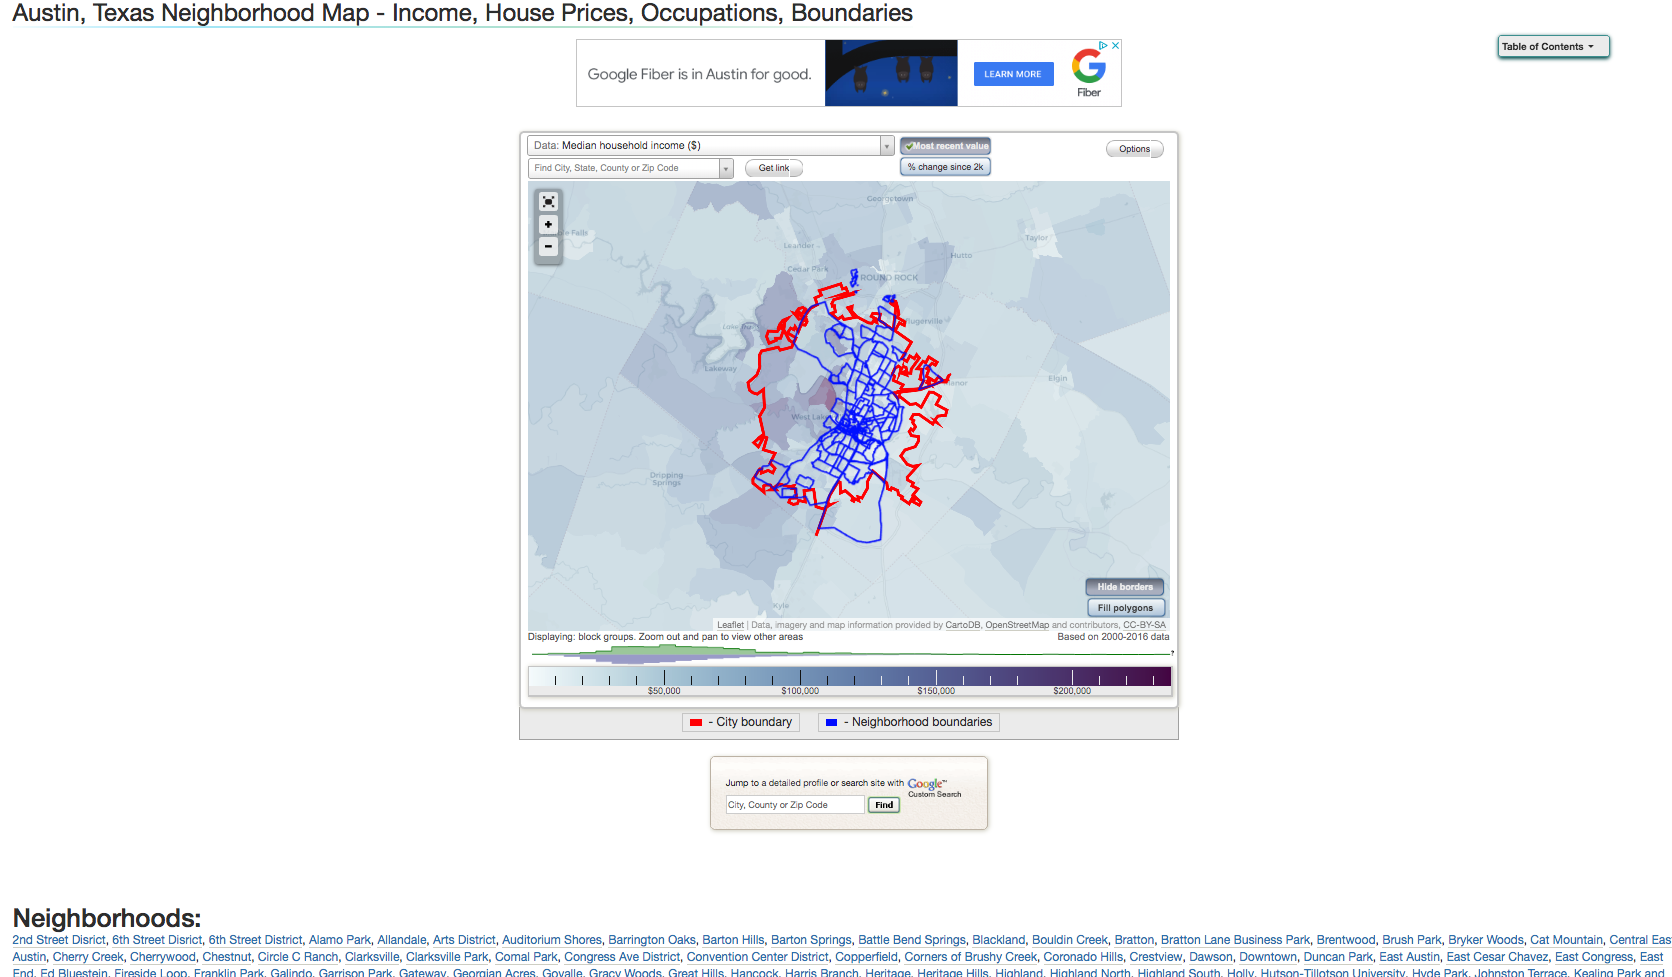
\includegraphics[width=.8\textwidth]{pics/city_data_start}
		\label{fig:1_1}
	\caption{City-Data webpage}
	\label{fig:4}
\end{figure}

While parsing this webpage, a part of the code detected and followed the links to a separate webpage for each neighborhood (see the list on the bottom of the webpage, as shown of Figure 2.) to obtain the information, such as neighborhood names, population, area and zipcodes. One can notice that some of these links contain more detailed information, including, for instance, residents' age and income. While such information can be useful for clustering analysis of the neighborhoods of Austin, for quite some of the neighborhoods this information was missing and it was decided to not use these features at all.

The obtained data was further transformed: a) features' values were casted into appropriate data types; b) neighborhoods sharing same zipcodes, were combined into one big neighborhood with population and area equal to the sum of all smaller ones.

The next step was to obtain geographical coordinates for each neighborhood. This was done straightforwardly using areaConnect website. For those neighborhoods, that correspond to several zipcodes, the resulting coordinates were computed as the average values. The resulting partitioning of the city into neighborhoods is illustrated on Figure 3.
%
\subsection{Venues data wrangling}
The neighborhoods data was scraped using requests and BeautifulSoup libraries. The starting point was the City-Data website main page, that looks as following:
\begin{figure}[H]
	\centering
	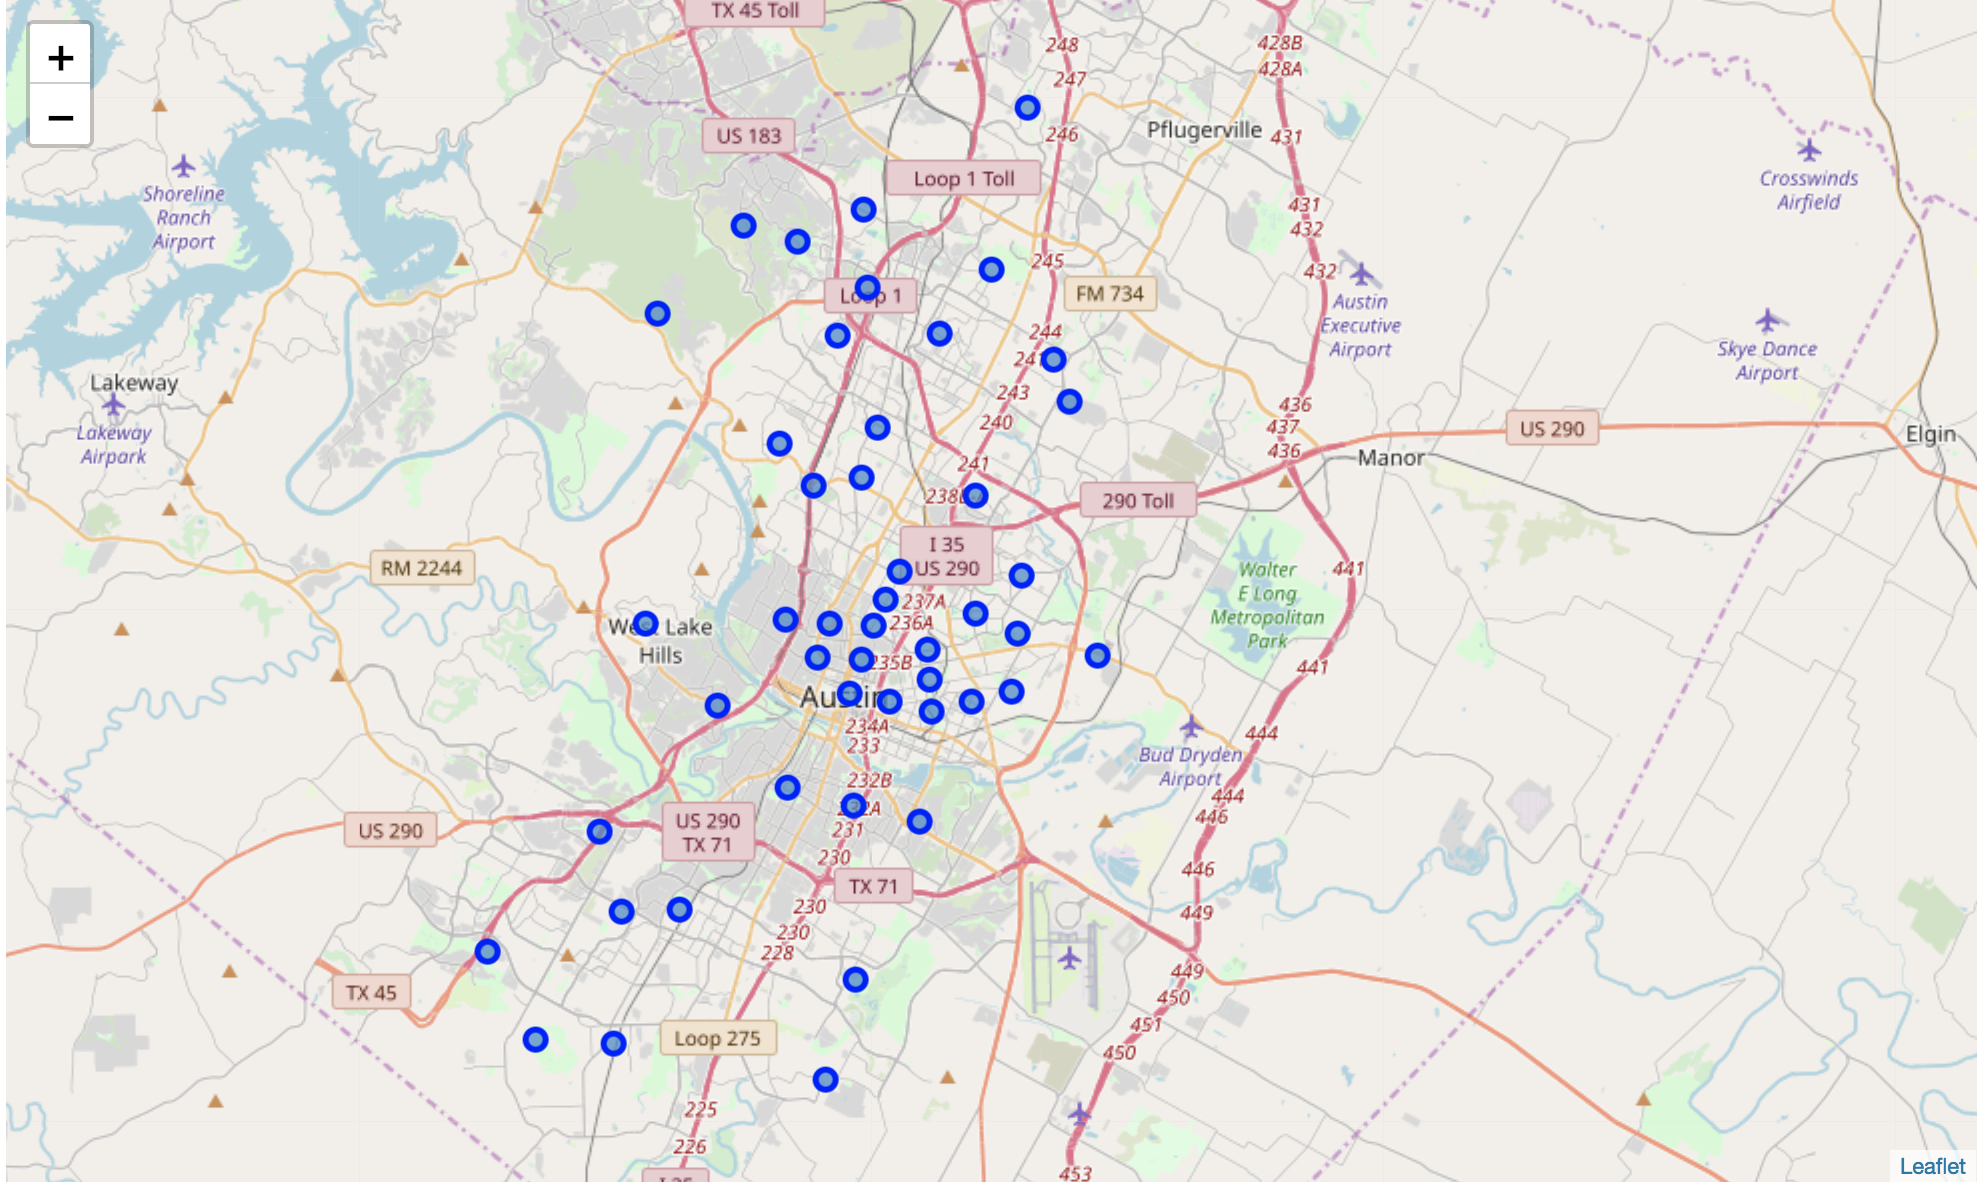
\includegraphics[width=.6\textwidth]{pics/neighborhoods}
		\label{fig:1_1}
	\caption{Centers of Austin's neighborhoods}
	\label{fig:4}
\end{figure}


The venues' information was scraped using calls to Foursquare API. For each of the neighborhoods, data about top 100 venues was downloaded, using the coordinates of the centers of the neighborhoods and the raduis, computed under the assumption that every neighborhood can be approximated as a circle. Such an assumption may not be very realistic, but, on the other hand, using a fixed value for the radius may lead to even more inaccuracy, since some of the neighborhoods are quite different in size. In order to account for the errors due the assumption, the radius was further adjusted by 20\%.

For each venue name, id, category and the corresponding geographical coordinates were stored. This data contained the information about all popular places, not limited to restaurants/food places, so the later were further picked out of all available data. Later in the analysis, after the candidate unusual categories of the restaurants were detected, customers' likes and venues' ratings were further downloaded using venue id for a small group of restaurants.

%%%%%%%%%%%%%%%%%%%%%%%%%%%%%%%%%%%%%%%%%%%%%%%%%%%%%%%%%%%%%%%%%%
\section{Methodology}
\subsection{Determine optimal venue category}
The first step of the analysis was to determine an attractive unusual restaurant category. For this purpose, for every neighborhood frequency of each type of cuisines/food places was computed, and, based on this, the top 20 and bottom 20 most frequent categories were identified. Figure 4 summarizes the resulting top and bottom venue types. 

Next, the venues from the least frequent categories were analyzed in more details. For each venue, the rating and customers' likes were added. The decision was made based on the top rated places with sufficient amount of likes, i.e., rating at least 8.0 and more than 50 likes. One particular category stood out in the resulting group of venues, {\bf Tapas Restaurant}: one out of two such venues had the highest ratings, while the other one had the second to largest amount of likes, as shown of Figure 5. Moreover, this category looked attractive as the goal was to determine a type of restaurants with elegant food and drinks in contrast to the everyone's favorite food trucks and taco places.
%
\begin{figure}[H]
	\centering
	\begin{subfigure}[b]{0.47\textwidth}
		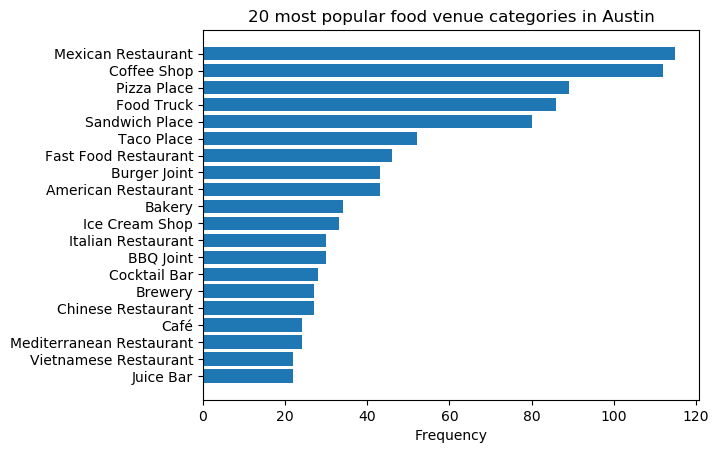
\includegraphics[width=\textwidth]{pics/top_20_venues}
		\caption{Top categories}
		\label{fig:1_1}
	\end{subfigure}
	\begin{subfigure}[b]{0.47\textwidth}
		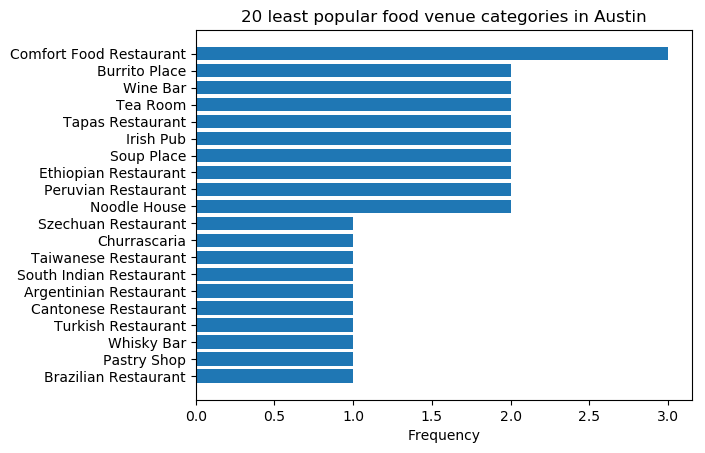
\includegraphics[width=\textwidth]{pics/bottom_20_venues}
		\caption{Bottom categories}
		\label{fig:1_2}
	\end{subfigure}
	\caption{The most and the least frequent venue types}
	\label{fig:3}
\end{figure}

\begin{figure}[H]
	\centering
	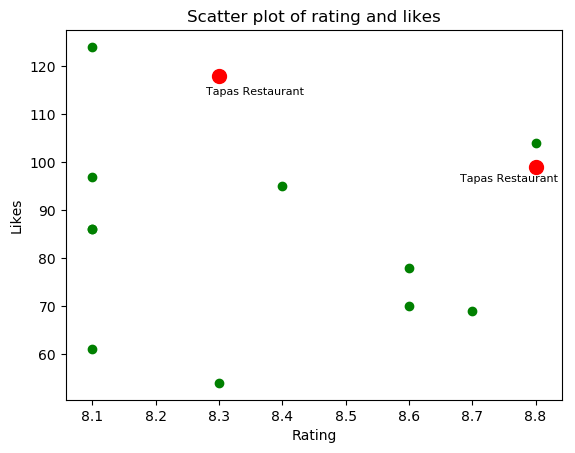
\includegraphics[width=.6\textwidth]{pics/ratings_and_likes}
		\label{fig:1_1}
	\caption{Ratings and likes for selected venues}
	\label{fig:4}
\end{figure}
%
\subsection{Choosing the best location}
After the best venue category was determined, it was left to suggest the optimal place to open a new restaurant. As it followed from the data, both Tapas Restaurants were located in the same neighborhood (see Figure 6). Clearly, opening another restaurant of the same, quite rare, category in the same neighborhoods would not be the smartest strategy. Therefore, the next step of the analysis was dedicated to studying the city neighborhoods.
\begin{figure}[H]
	\centering
	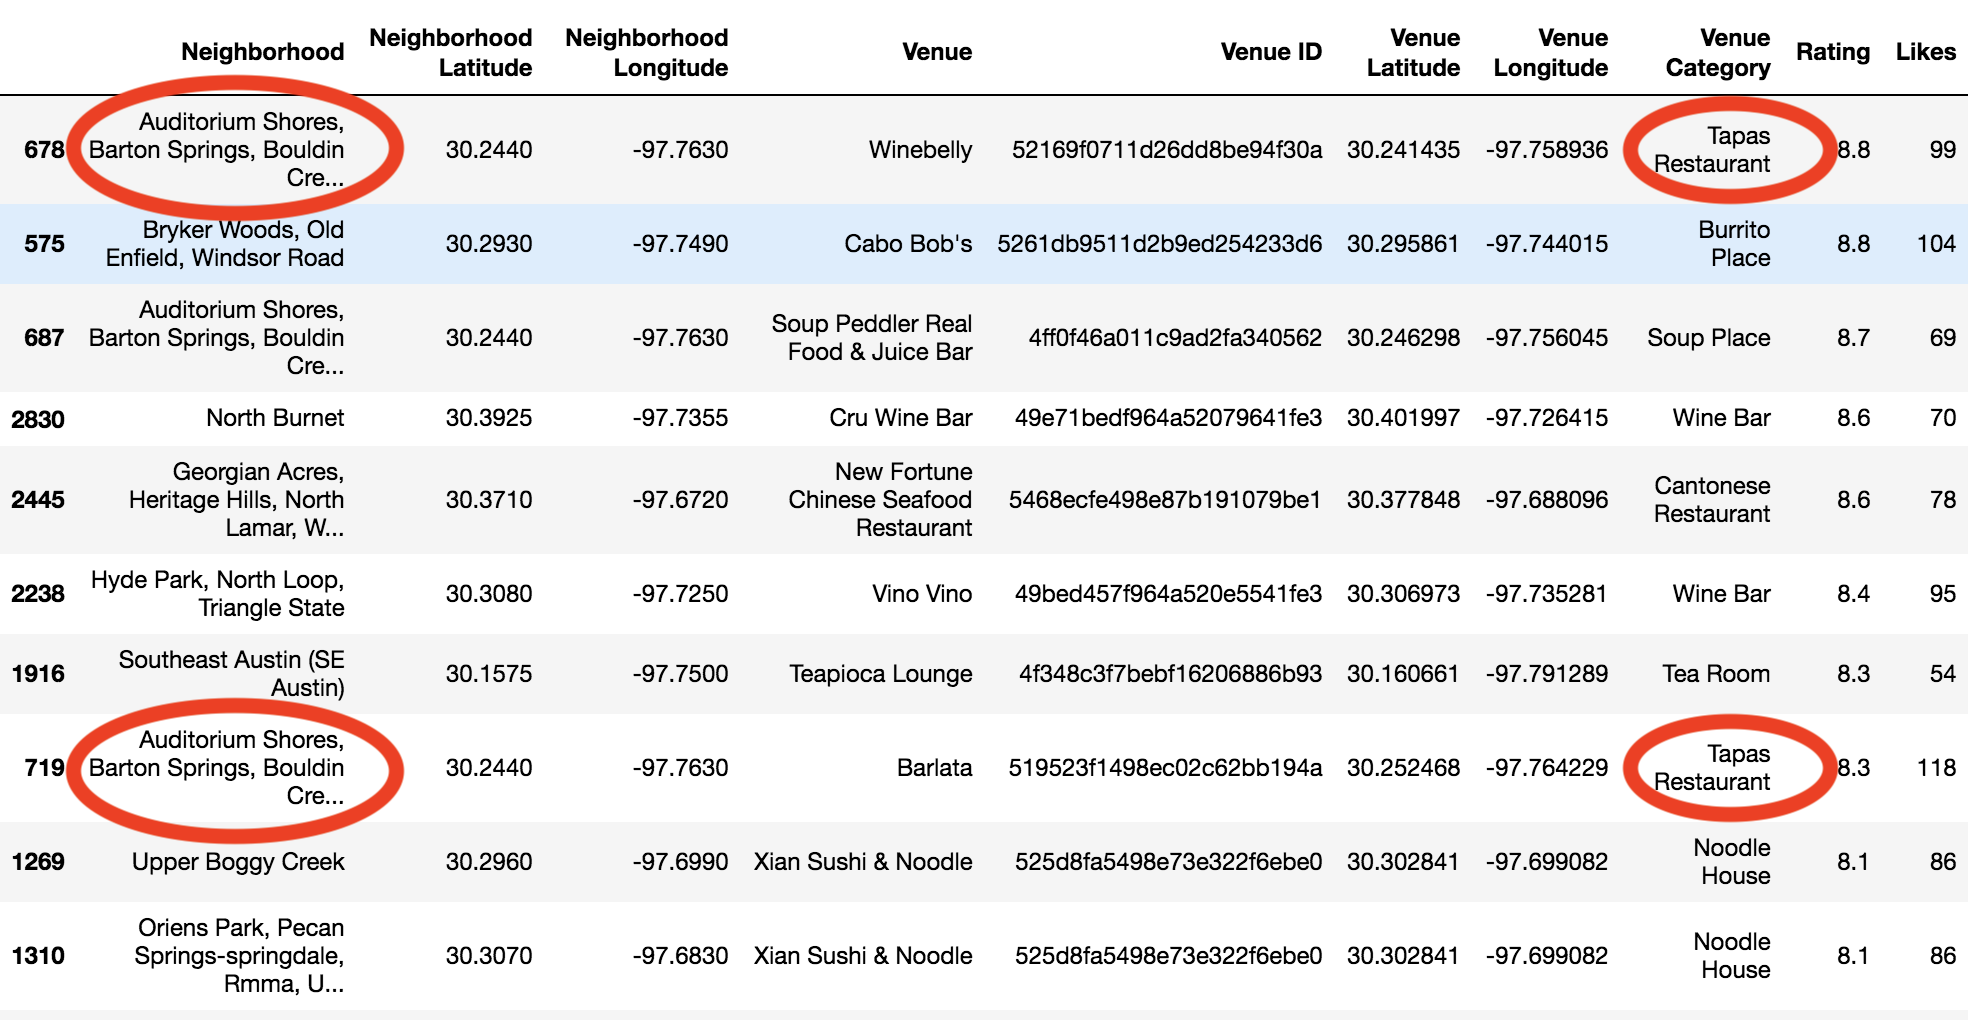
\includegraphics[width=.9\textwidth]{pics/top_10_rare}
		\label{fig:1_1}
	\caption{Top 10 venues from rare categories, sorted by rating}
	\label{fig:4}
\end{figure}
%
To measure the  similarity between neighborhoods, the clustering analysis, using k-means algorithm, was performed. The features included the frequencies of all possible popular venues (not limited to restaurants, as in the previous subsection), as well as population and area of each neighborhood. Below are the results of clustering of 48 Austin's neighborhoods using k-means with $k=7$. The neighborhood that already has two Tapas Restaurants is marked by a red circle.
\begin{figure}[H]
	\centering
	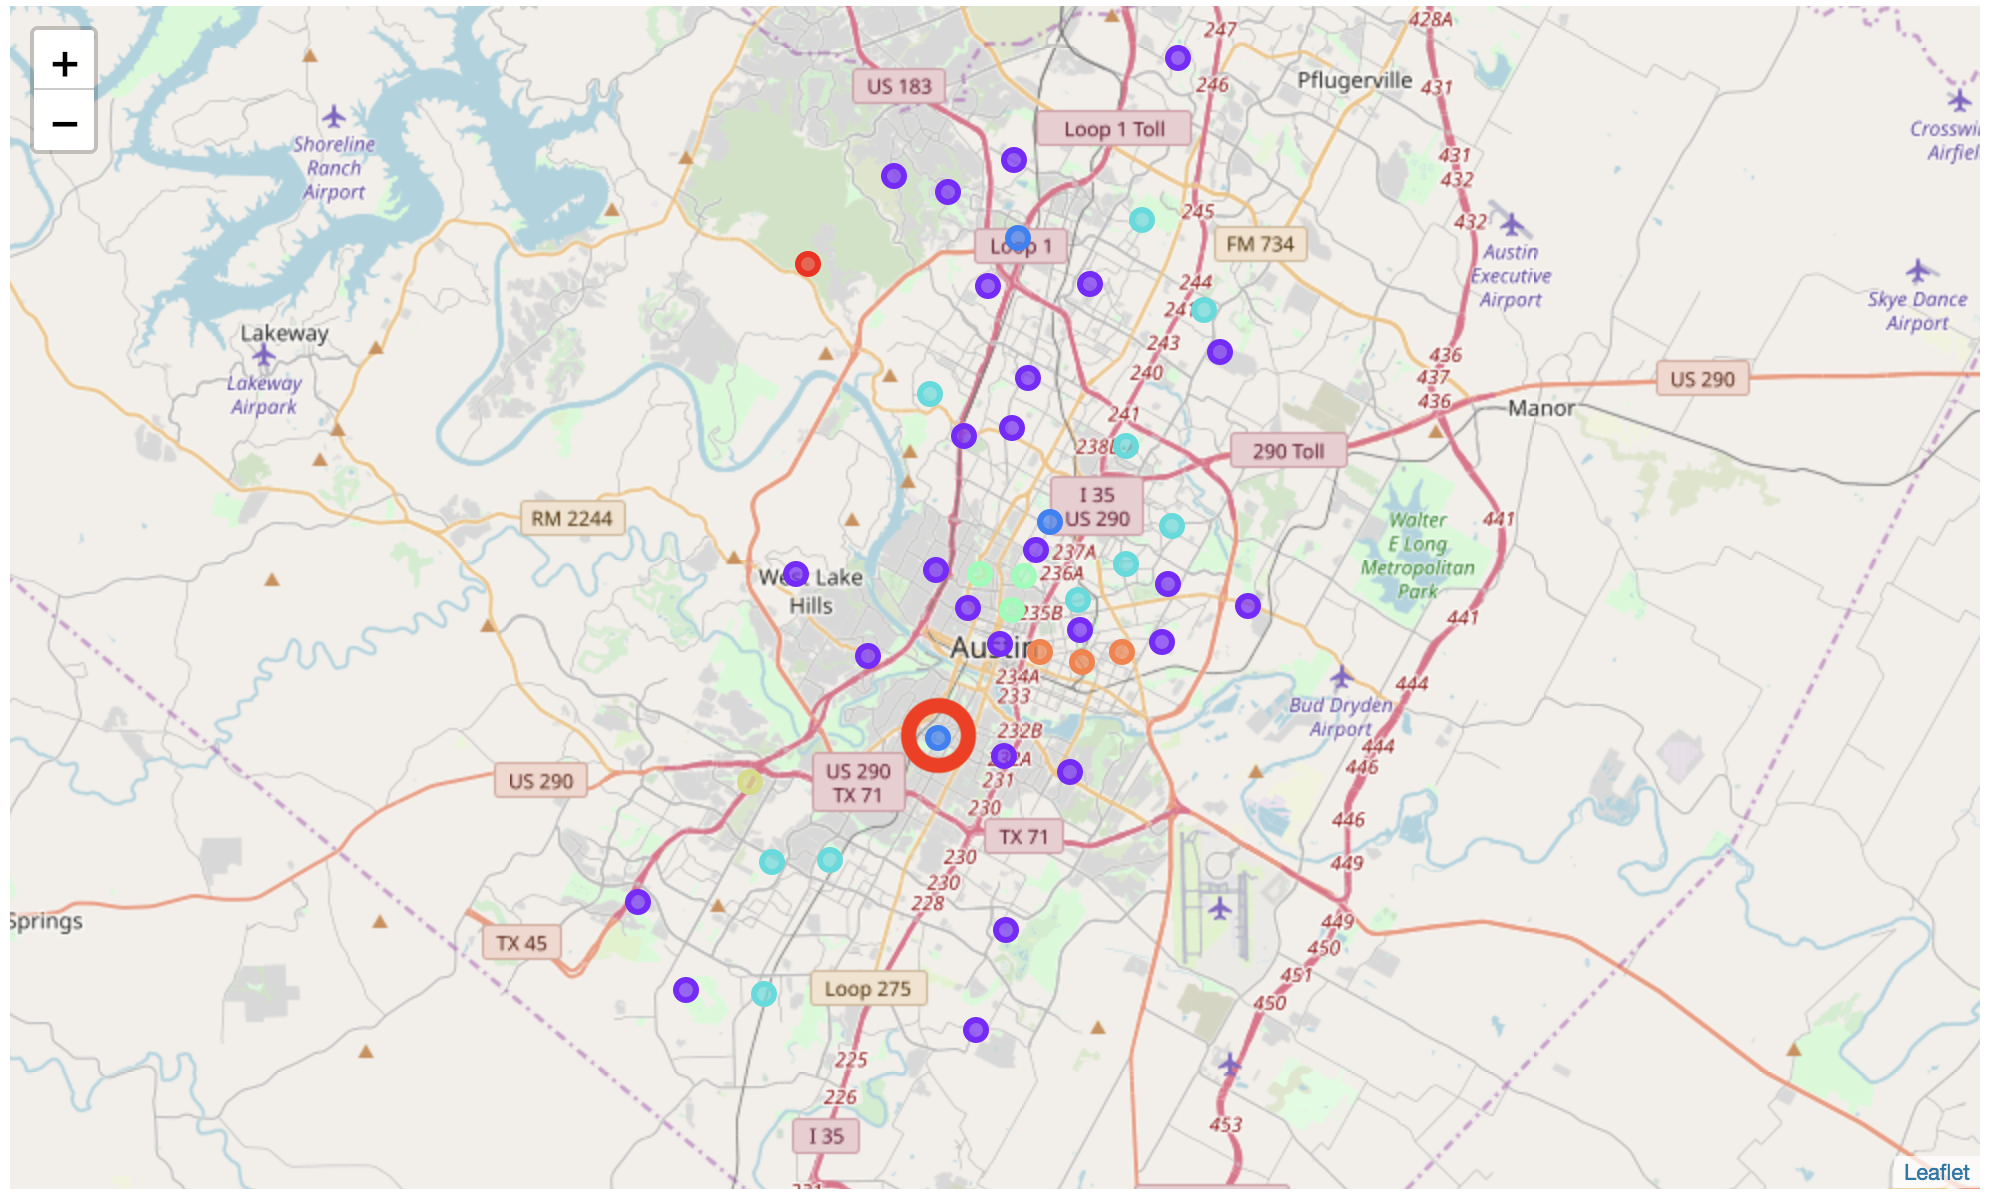
\includegraphics[width=.9\textwidth]{pics/clusters}
		\label{fig:1_1}
	\caption{Clusters of Austin's neighborhoods}
	\label{fig:4}
\end{figure}
The cluster of interest contains 3 neighborhoods, including the one with existing Tapas Restaurants. Hence, based on this analysis, the other two neighborhoods are optimal for opening a new restaurant of this category. These neighborhoods (consisting of smaller ones) include:
{\bf
\begin{itemize}
\item \begin{itemize}
\item Hyde Park
\item North Loop
\item Triangle State
\end{itemize}
\item North Burnet
\end{itemize}
}

%%%%%%%%%%%%%%%%%%%%%%%%%%%%%%%%%%%%%%%%%%%%%%%%%%%%%%%%%%%%%%%%%%
\section{Results and Discussion}
Based on the performed analysis, the best category turned out to be a {\bf Tapas Restaurant} and the optimal location - one of the two neighborhoods:
{\bf
\begin{itemize}
\item \begin{itemize}
\item Hyde Park
\item North Loop
\item Triangle State
\end{itemize}
\item North Burnet
\end{itemize}
}

The choice of restaurant type seems reasonable. First of all, it is suitable both as an upscale food destination for the tourists, as well as the locals, who would like to try something unusual. Moreover, since the Spanish cuisine is up to some extend close to the Mexican cuisine, such a restaurant would still posses some of the flavour of the local famous and favorite food. Therefore, a Tapas Restaurant fit nicely, provided one chooses the location optimally.

According to the available data, there are currently two Tapas Restaurants in Austin, both located in the same neighborhood. In order not to get unnoticed when opening a new restaurant and to avoid competition with the existing places, the new restaurant should be opened in another neighborhood, which nevertheless posses similarities with the one that has the restaurants. As the results of the clustering analysis, it was determined that the neighborhoods with existing restaurants forms a cluster with two other ones, which are, therefore, a good choice for the new restaurant location.  Interestingly, there are {\it Wine Bars} in both of these neighborhoods, which can be viewed as good sign, since this category is quite close to the the Tapas Restaurants and, hence, the new restaurant should be of interest for the residents.

Although, the conclusion based on the performed analysis seems persuasive enough, there are several inaccuracies, that may introduce errors and lead to misleading results:
\begin{itemize}
\item The neighborhoods were represented geometrically as circles, based on the area, and the radius of each circle (with some adjustments) was used to the Foursquare calls. Clearly, such assumption doesn't sound very realistic, as the neighborhoods can be irregularly shaped. However, a more accurate procedure seems to be unavailable, since Foursquare calls use geographical coordinates of the center of a neighborhood and a radius.
\item The neighborhoods sharing same zipcode were combined into bigger ones and the corresponding coordinated were computed as the average values. Although, this might be inaccurate and introduce some errors into the analysis, a more accurate geographical segmentation of the city is out of the scope of this project.
\end{itemize}
Finally, one possible improvement can be based on gathering more data the neighborhoods and their population statistics, including average resident's age, income and so on. Such detailed information might improve the segmentation accuracy.
%%%%%%%%%%%%%%%%%%%%%%%%%%%%%%%%%%%%%%%%%%%%%%%%%%%%%%%%%%%%%%%%%%
\section{Conclusions}
In this project the analysis of Austin's neighborhoods and available restaurants was performed. According to the data, the most popular venue types include Mexican Restaurants, Coffee Shops, Pizza Restaurants and other, while the places such as Tapas Restaurants, Wine Bars, and exotic cuisines, such as Ethiopian and Peruvian, are not very common. Based on the current demographic trends and the information about existing food venues, it was concluded that a Tapas Restaurant would be a perfect food venue category for a new restaurant. It was further shown through the segmentation of Austin's neighborhoods that there are certain locations that are the most suitable for such new restaurant. The project was summed up by discussing the results, pointing out existing weaknesses, as well as possible improvements. 
%%%%%%%%%%%%%%%%%%%%%%%%%%%%%%%%%%%%%%%%%%%%%%%%%%%%%%%%%%%%%%%%%%
\begin{thebibliography}{1}
   \bibitem{census} https://www.census.gov/newsroom/press-releases/2019/estimates-county-metro.html
    \bibitem{culture_map} http://austin.culturemap.com/news/city-life/01-09-19-population-of-austin-prepared-to-pop-to-1-million-in-2020/
     \bibitem{realestate}https://realestate.usnews.com/places/texas/austin
     \bibitem{zagat} https://www.zagat.com/b/30-most-exciting-food-cities-in-america-2017
      \bibitem{foursquare} https://developer.foursquare.com/
      \bibitem{city_data} http://www.city-data.com/nbmaps/neigh-Austin-Texas.html\#N22
      \bibitem{area_connect}http://austintx.areaconnect.com/zip2.htm?city=Austin\&qs=TX\&searchtype=bycity
  \end{thebibliography}
\end{document} 
